\section[Image Processing]{Image Processing}

\begin{frame}{Application to Image Processing}
	In this section, we will explore:
	\begin{itemize}
		\item How a machine learning algorithm processes image-type data.
		\item How the Principal Component Analysis method can be utilized to simplify a problem that uses images as inputs.
	\end{itemize}
\end{frame}

\subsection[Image Representation]{Image Representation}

\begin{frame}{From Image to Vector (Flattening)}
	To understand how an algorithm processes a \textbf{black and white} (binary) image, let us look at a simplified example: a \textbf{"0"} displayed on a $5 \times 3$ pixel grid.
	\begin{figure}
		\centering
		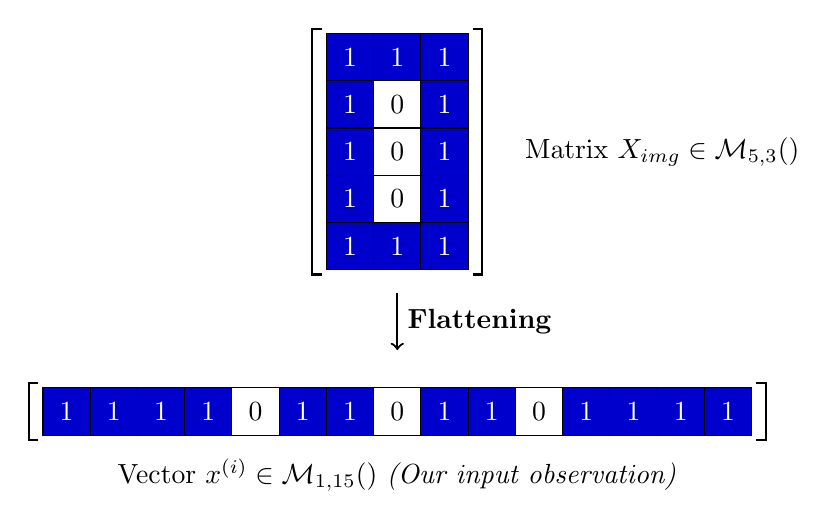
\begin{tikzpicture}[scale=0.6, every node/.style={minimum size=0.6cm}]
			% Color definitions for pixels (dark blue for 1, white for 0)
			\colorlet{pixelon}{blue!80!black}
			\colorlet{pixeloff}{white}
			
			% --- 5x3 MATRIX (Centered top) ---
			\begin{scope}[xshift=-1cm] 
				% Row 1
				\node[draw, fill=pixelon, text=white] at (0, 4) {1};
				\node[draw, fill=pixelon, text=white] at (1, 4) {1};
				\node[draw, fill=pixelon, text=white] at (2, 4) {1};
				% Row 2
				\node[draw, fill=pixelon, text=white] at (0, 3) {1};
				\node[draw, fill=pixeloff, text=black] at (1, 3) {0};
				\node[draw, fill=pixelon, text=white] at (2, 3) {1};
				% Row 3
				\node[draw, fill=pixelon, text=white] at (0, 2) {1};
				\node[draw, fill=pixeloff, text=black] at (1, 2) {0};
				\node[draw, fill=pixelon, text=white] at (2, 2) {1};
				% Row 4
				\node[draw, fill=pixelon, text=white] at (0, 1) {1};
				\node[draw, fill=pixeloff, text=black] at (1, 1) {0};
				\node[draw, fill=pixelon, text=white] at (2, 1) {1};
				% Row 5
				\node[draw, fill=pixelon, text=white] at (0, 0) {1};
				\node[draw, fill=pixelon, text=white] at (1, 0) {1};
				\node[draw, fill=pixelon, text=white] at (2, 0) {1};
				
				% Matrix brackets
				\draw[thick] (-0.6, -0.6) -- (-0.8, -0.6) -- (-0.8, 4.6) -- (-0.6, 4.6);
				\draw[thick] (2.6, -0.6) -- (2.8, -0.6) -- (2.8, 4.6) -- (2.6, 4.6);
			\end{scope}
			
			% Text next to the matrix
			\node[right] at (2.5, 2) {Matrix $X_{\text{img}} \in \mathcal{M}_{5,3}(\R)$};
			
			% --- FLATTENING ARROW ---
			\draw[->, thick] (0, -1) -- (0, -2.2) node[midway, right] {\textbf{Flattening}};
			
			% --- 1x15 VECTOR (Row-by-row flattening) ---
			\begin{scope}[xshift=-7cm, yshift=-3.5cm]
				\node[draw, fill=pixelon, text=white] at (0, 0) {1};
				\node[draw, fill=pixelon, text=white] at (1, 0) {1};
				\node[draw, fill=pixelon, text=white] at (2, 0) {1};
				
				\node[draw, fill=pixelon, text=white] at (3, 0) {1};
				\node[draw, fill=pixeloff, text=black] at (4, 0) {0};
				\node[draw, fill=pixelon, text=white] at (5, 0) {1};
				
				\node[draw, fill=pixelon, text=white] at (6, 0) {1};
				\node[draw, fill=pixeloff, text=black] at (7, 0) {0};
				\node[draw, fill=pixelon, text=white] at (8, 0) {1};
				
				\node[draw, fill=pixelon, text=white] at (9, 0) {1};
				\node[draw, fill=pixeloff, text=black] at (10, 0) {0};
				\node[draw, fill=pixelon, text=white] at (11, 0) {1};
				
				\node[draw, fill=pixelon, text=white] at (12, 0) {1};
				\node[draw, fill=pixelon, text=white] at (13, 0) {1};
				\node[draw, fill=pixelon, text=white] at (14, 0) {1};
				
				% Vector brackets
				\draw[thick] (-0.6, -0.6) -- (-0.8, -0.6) -- (-0.8, 0.6) -- (-0.6, 0.6);
				\draw[thick] (14.6, -0.6) -- (14.8, -0.6) -- (14.8, 0.6) -- (14.6, 0.6);
				
				% Legend under the vector
				\node[below] at (7, -0.8) {Vector $x^{(i)} \in \mathcal{M}_{1,15}(\R)$ \textit{(Our input observation)}};
			\end{scope}
		\end{tikzpicture}
	\end{figure}
\end{frame}

\begin{frame}{From Image to Vector (Flattening)}
	Here is another example featuring a \textbf{"4"}:
	\begin{figure}
		\centering
		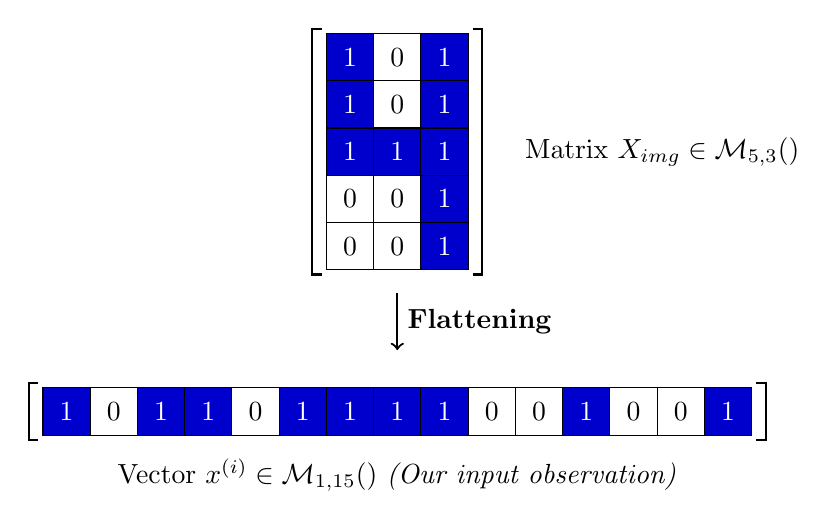
\begin{tikzpicture}[scale=0.6, every node/.style={minimum size=0.6cm}]
			% Color definitions for pixels (dark blue for 1, white for 0)
			\colorlet{pixelon}{blue!80!black}
			\colorlet{pixeloff}{white}
			
			% --- 5x3 MATRIX (Centered top) ---
			\begin{scope}[xshift=-1cm] 
				% Row 1
				\node[draw, fill=pixelon, text=white] at (0, 4) {1};
				\node[draw, fill=pixeloff, text=black] at (1, 4) {0};
				\node[draw, fill=pixelon, text=white] at (2, 4) {1};
				% Row 2
				\node[draw, fill=pixelon, text=white] at (0, 3) {1};
				\node[draw, fill=pixeloff, text=black] at (1, 3) {0};
				\node[draw, fill=pixelon, text=white] at (2, 3) {1};
				% Row 3
				\node[draw, fill=pixelon, text=white] at (0, 2) {1};
				\node[draw, fill=pixelon, text=white] at (1, 2) {1};
				\node[draw, fill=pixelon, text=white] at (2, 2) {1};
				% Row 4
				\node[draw, fill=pixeloff, text=black] at (0, 1) {0};
				\node[draw, fill=pixeloff, text=black] at (1, 1) {0};
				\node[draw, fill=pixelon, text=white] at (2, 1) {1};
				% Row 5
				\node[draw, fill=pixeloff, text=black] at (0, 0) {0};
				\node[draw, fill=pixeloff, text=black] at (1, 0) {0};
				\node[draw, fill=pixelon, text=white] at (2, 0) {1};
				
				% Matrix brackets
				\draw[thick] (-0.6, -0.6) -- (-0.8, -0.6) -- (-0.8, 4.6) -- (-0.6, 4.6);
				\draw[thick] (2.6, -0.6) -- (2.8, -0.6) -- (2.8, 4.6) -- (2.6, 4.6);
			\end{scope}
			
			% Text next to the matrix
			\node[right] at (2.5, 2) {Matrix $X_{\text{img}} \in \mathcal{M}_{5,3}(\R)$};
			
			% --- FLATTENING ARROW ---
			\draw[->, thick] (0, -1) -- (0, -2.2) node[midway, right] {\textbf{Flattening}};
			
			% --- 1x15 VECTOR (Row-by-row flattening) ---
			\begin{scope}[xshift=-7cm, yshift=-3.5cm]
				\node[draw, fill=pixelon, text=white] at (0, 0) {1};
				\node[draw, fill=pixeloff, text=black] at (1, 0) {0};
				\node[draw, fill=pixelon, text=white] at (2, 0) {1};
				
				\node[draw, fill=pixelon, text=white] at (3, 0) {1};
				\node[draw, fill=pixeloff, text=black] at (4, 0) {0};
				\node[draw, fill=pixelon, text=white] at (5, 0) {1};
				
				\node[draw, fill=pixelon, text=white] at (6, 0) {1};
				\node[draw, fill=pixelon, text=white] at (7, 0) {1};
				\node[draw, fill=pixelon, text=white] at (8, 0) {1};
				
				\node[draw, fill=pixeloff, text=black] at (9, 0) {0};
				\node[draw, fill=pixeloff, text=black] at (10, 0) {0};
				\node[draw, fill=pixelon, text=white] at (11, 0) {1};
				
				\node[draw, fill=pixeloff, text=black] at (12, 0) {0};
				\node[draw, fill=pixeloff, text=black] at (13, 0) {0};
				\node[draw, fill=pixelon, text=white] at (14, 0) {1};
				
				% Vector brackets
				\draw[thick] (-0.6, -0.6) -- (-0.8, -0.6) -- (-0.8, 0.6) -- (-0.6, 0.6);
				\draw[thick] (14.6, -0.6) -- (14.8, -0.6) -- (14.8, 0.6) -- (14.6, 0.6);
				
				% Legend under the vector
				\node[below] at (7, -0.8) {Vector $x^{(i)} \in \mathcal{M}_{1,15}(\R)$ \textit{(Our input observation)}};
			\end{scope}
		\end{tikzpicture}
	\end{figure}
\end{frame}

\begin{frame}{Grayscale Images}
	A grayscale image with a resolution of 1280 x 720 pixels (commonly known as HD resolution):
	\begin{itemize}
		\item Is represented in a computer by a 720 by 1280 matrix. When discussing resolution, we state width x height, whereas the matrix maps width to columns and height to rows. This can be misleading!
		\item Each element of the matrix contains an integer ranging from 0 to 255 ($2^8$, i.e., 8 bits):
		\begin{itemize}
			\item 0: The pixel will be completely black.
			\item 255: The pixel will be completely white.
			\item Intermediate values represent various shades of gray.
		\end{itemize}
		\item For machine learning algorithms, pixels are usually normalized so that their values fall between 0 and 1.
		\item Such an image represents an input space with a dimensionality of roughly 0.9 million: $720 \times 1280 = 921600$.
	\end{itemize}
\end{frame}

\begin{frame}{Color Images}
	A color image with a resolution of 1280 x 720 pixels, designated as RGB (Red / Green / Blue):
	\begin{itemize}
		\item Is represented in a computer by 3 distinct matrices of size 720 by 1280, one for each color channel (red, green, or blue). It is also referred to as a \textbf{tensor} of dimensions 720 x 1280 x 3.
		\item Each matrix element contains an integer between 0 and 255 ($2^8$, i.e., 8 bits):
		\begin{itemize}
			\item 0: No intensity for the current color channel.
			\item 255: Maximum intensity for the current color channel.
			\item Intermediate values represent varying levels of intensity for that color.
		\end{itemize}
		\item For machine learning algorithms, pixels are normalized so that their values lie between 0 and 1.
		\item Such an image is capable of displaying 16 million colors: $256 \times 256 \times 256 = 16777216$.
		\item This image therefore represents an input space with a dimensionality of 2.7 million: $720 \times 1280 \times 3 = 2764800$.
	\end{itemize}
\end{frame}

\begin{frame}{Image Examples}
	\begin{figure}
		\centering
		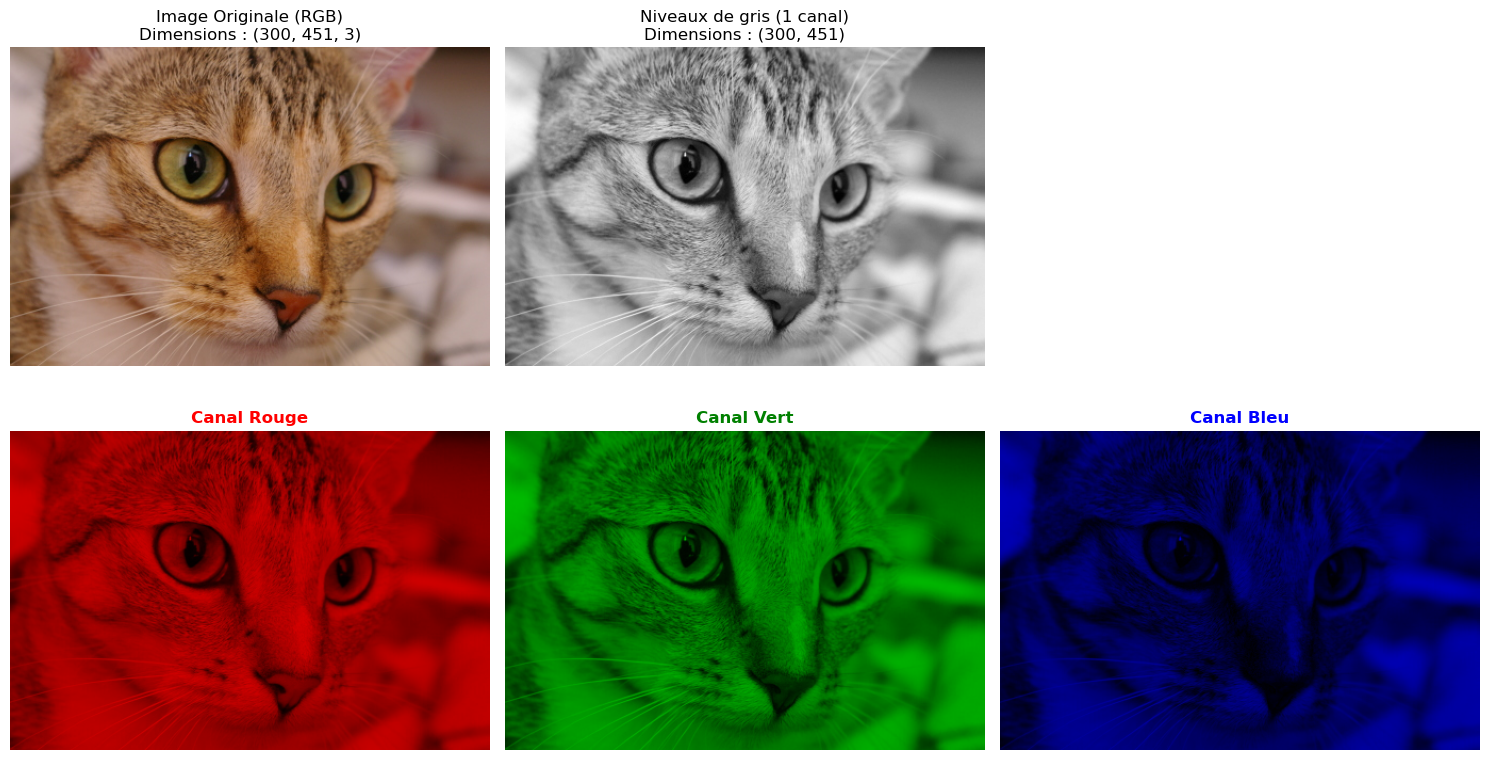
\includegraphics[width=1.0\linewidth]{Images/chelsea}
		\label{fig:chelsea}
	\end{figure}
\end{frame}

\begin{frame}{Image Examples}
	\begin{figure}
		\centering
		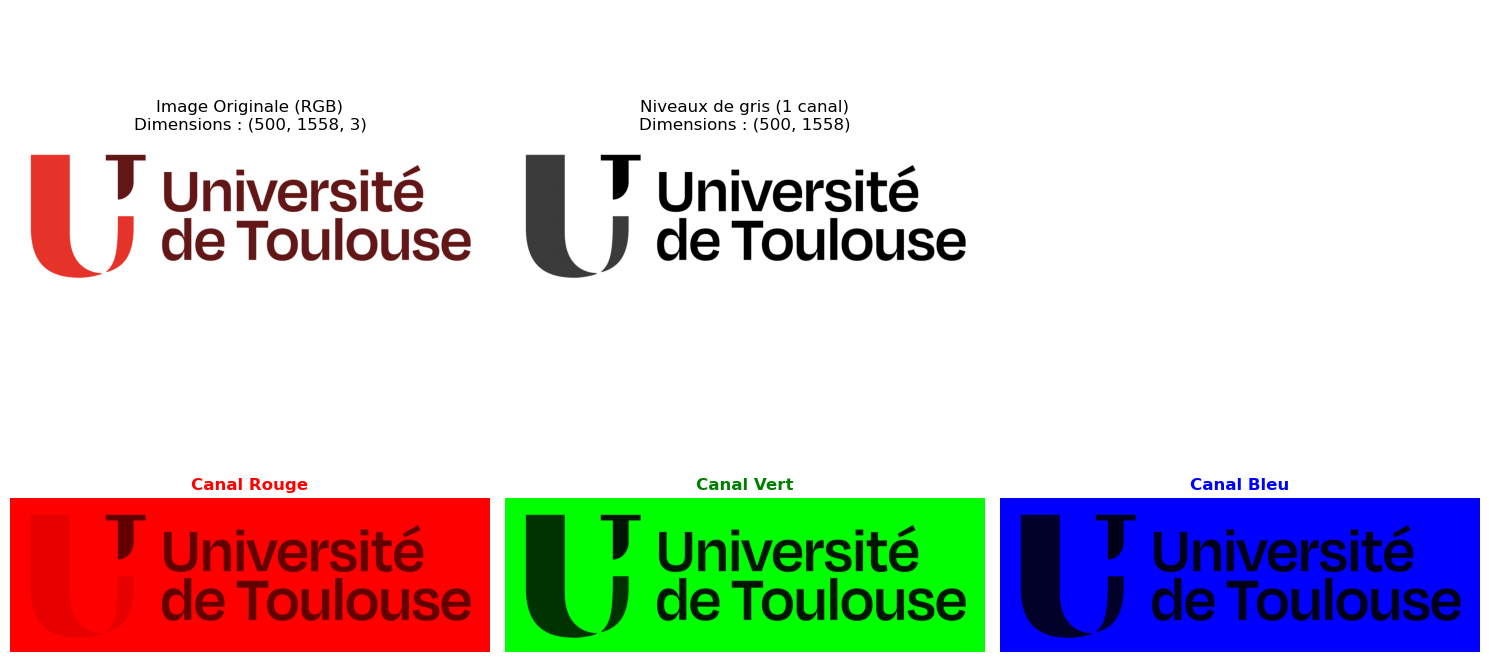
\includegraphics[width=1.0\linewidth]{Images/logo-UT-RGB}
		\label{fig:logo-UT-RGB}
	\end{figure}
\end{frame}

\subsection[PCA Applied to Images]{PCA Applied to Images}

\begin{frame}{Case Study}
	In this section, we will apply Principal Component Analysis to images. As previously demonstrated, images serve as high-dimensional inputs. Consequently, any form of dimensionality reduction is highly valuable before feeding these images into a regression or classification algorithm. \\
	\pause
	\vspace{0.5cm}
	We will use the MNIST dataset as our benchmark, which contains grayscale images of handwritten digits: \href{https://www.kaggle.com/datasets/hojjatk/mnist-dataset}{\textbf{Kaggle MNIST Dataset}}.
	\begin{itemize}
		\item Yann LeCun, Courant Institute, NYU
		\item Corinna Cortes, Google Labs, New York
		\item Christopher J.C. Burges, Microsoft Research, Redmond
	\end{itemize}
\end{frame}

\begin{frame}{Image Examples}
	The images feature a resolution of $28 \times 28 = 784$ pixels and are provided in grayscale. Here are a few examples:
	\begin{columns}
		\begin{column}{0.33\textwidth}
			\begin{figure}
				\centering
				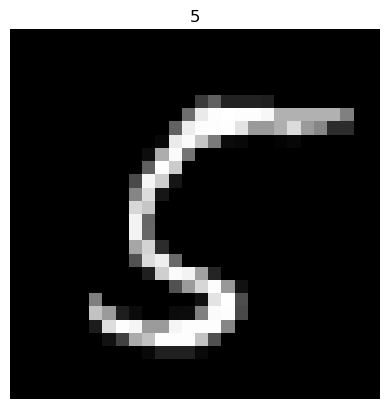
\includegraphics[width=1.0\linewidth]{Images/MNIST-5}
				\label{fig:MNIST-5}
			\end{figure}			
		\end{column}
		\begin{column}{0.33\textwidth}
			\begin{figure}
				\centering
				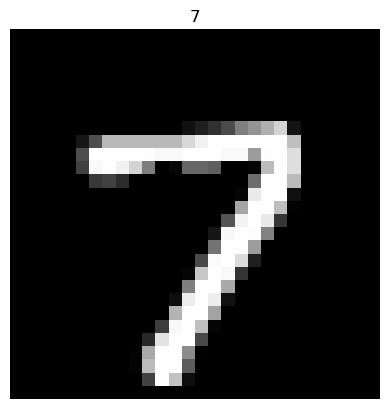
\includegraphics[width=1.0\linewidth]{Images/MNIST-7}
				\label{fig:MNIST-7}
			\end{figure}						
		\end{column}
		\begin{column}{0.33\textwidth}
			\begin{figure}
				\centering
				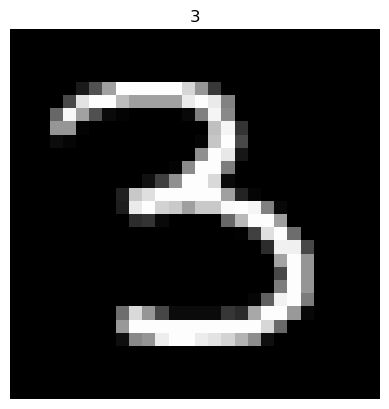
\includegraphics[width=1.0\linewidth]{Images/MNIST-3}
				\label{fig:MNIST-3}
			\end{figure}			
		\end{column}
	\end{columns}
\end{frame}

\begin{frame}{Image Processing with PCA}
	Each image is therefore treated as a row vector containing 784 values! Here is the workflow applied to the images:
	\begin{enumerate}
		\item First, we normalize the data. Since each pixel ranges from 0 to 255, we divide all terms by 255. While not strictly mandatory, this keeps the resulting eigenvalues relatively small.
		\item We center the dataset by subtracting the mean image from each individual image.
		\item Exceptionally, we do not divide by the variance: a pixel located in the corner of the image has a very high probability of remaining black across the dataset, yielding a variance of zero. Since all pixels share a similar scale, centering is sufficient, even though the variance of each pixel is not unit.
		\item We compute all eigenvalues and eigenvectors using: \href{https://scikit-learn.org/stable/modules/generated/sklearn.decomposition.PCA.html}{\texttt{sklearn.decomposition.PCA}}.
		\item This enables us to plot the eigenvalue scree plot.
	\end{enumerate}
\end{frame}

\begin{frame}{Eigenvalue Scree Plot for the MNIST Dataset}
	\begin{columns}
		\begin{column}{0.7\textwidth}
			\begin{figure}
				\centering
				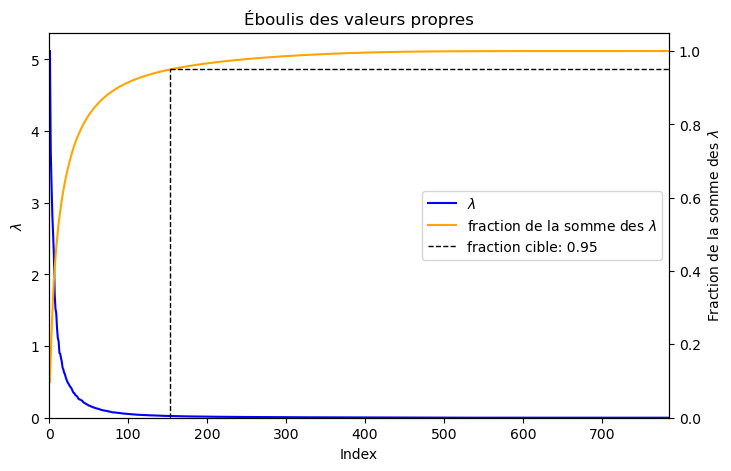
\includegraphics[width=1.0\linewidth]{Images/eboulis-MNIST}
				\label{fig:eboulis-MNIST}
			\end{figure}			
		\end{column}
		\begin{column}{0.3\textwidth}
			We can retain 95\% of the total dataset variance by keeping only the top 150 largest eigenvalues! This reduces the dimensionality of the problem by a factor of 5.
		\end{column}
	\end{columns}
\end{frame}

\begin{frame}{Retaining All Components}
	By retaining 100\% of the components, the reconstructed image ($\hat{x}^{(i)}$) is perfect. The error matrix $x^{(i)} - \hat{x}^{(i)}$ is completely zero. This confirms that PCA successfully redistributes variance without any loss of information:
	\begin{columns}
		\begin{column}{0.25\textwidth}
			\begin{figure}
				\centering
				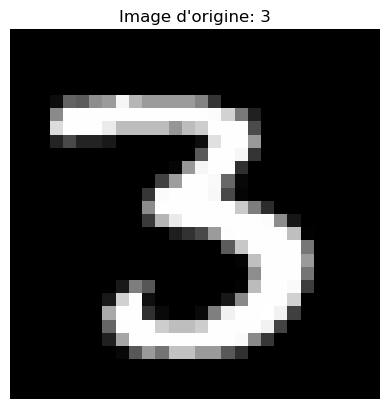
\includegraphics[width=1.0\linewidth]{Images/MNIST-3-28-origine}
				\label{fig:MNIST-3-28-origine}
			\end{figure}						
		\end{column}
		\begin{column}{0.25\textwidth}
			\begin{figure}
				\centering
				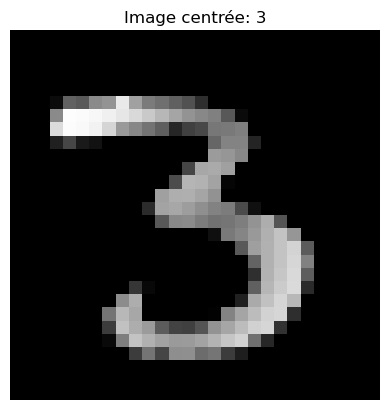
\includegraphics[width=1.0\linewidth]{Images/MNIST-3-28-centree}
				\label{fig:MNIST-3-28-centree}
			\end{figure}						
		\end{column}
		\begin{column}{0.25\textwidth}
			\begin{figure}
				\centering
				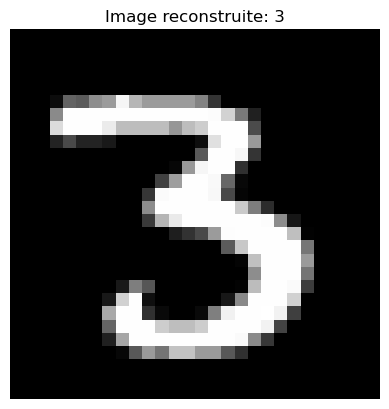
\includegraphics[width=1.0\linewidth]{Images/MNIST-3-28-reconstruite}
				\label{fig:MNIST-3-28-reconstruite}
			\end{figure}						
		\end{column}
		\begin{column}{0.25\textwidth}
			\begin{figure}
				\centering
				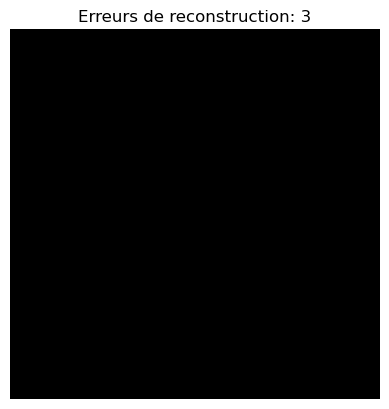
\includegraphics[width=1.0\linewidth]{Images/MNIST-3-28-erreur}
				\label{fig:MNIST-3-28-erreur}
			\end{figure}						
		\end{column}
	\end{columns}
\end{frame}

\begin{frame}{Retaining the Top 144 Components}
	Our cumulative variance scree plot suggested that with roughly 150 components, 95\% of the variance is preserved. The reconstructed image, though imperfect, is still easily recognizable as a \textbf{"3"}. The error plot highlights a minor discrepancy localized within a very specific area of the image during reconstruction:
	\begin{columns}
		\begin{column}{0.25\textwidth}
			\begin{figure}
				\centering
				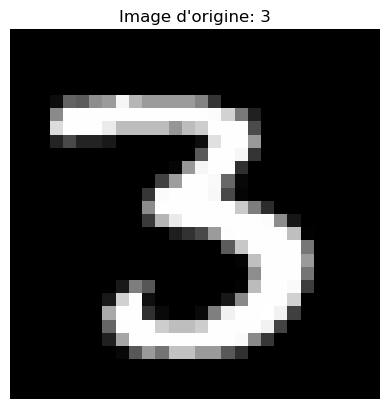
\includegraphics[width=1.0\linewidth]{Images/MNIST-3-12-origine}
				\label{fig:MNIST-3-12-origine}
			\end{figure}						
		\end{column}
		\begin{column}{0.25\textwidth}
			\begin{figure}
				\centering
				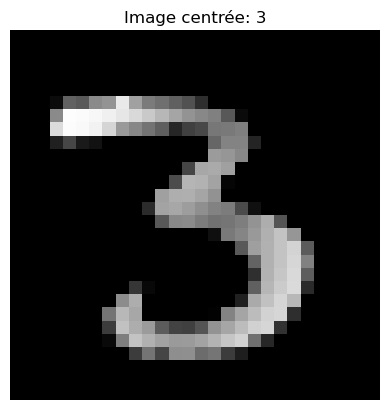
\includegraphics[width=1.0\linewidth]{Images/MNIST-3-12-centree}
				\label{fig:MNIST-3-12-centree}
			\end{figure}						
		\end{column}
		\begin{column}{0.25\textwidth}
			\begin{figure}
				\centering
				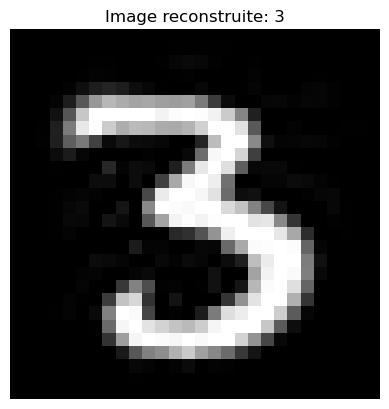
\includegraphics[width=1.0\linewidth]{Images/MNIST-3-12-reconstruite}
				\label{fig:MNIST-3-12-reconstruite}
			\end{figure}						
		\end{column}
		\begin{column}{0.25\textwidth}
			\begin{figure}
				\centering
				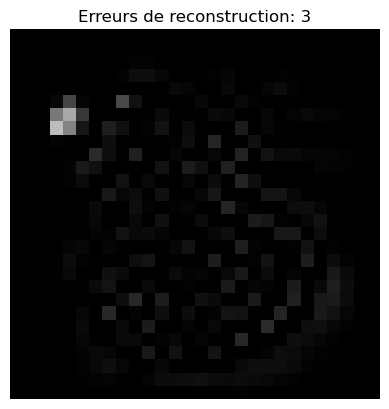
\includegraphics[width=1.0\linewidth]{Images/MNIST-3-12-erreur}
				\label{fig:MNIST-3-12-erreur}
			\end{figure}						
		\end{column}
	\end{columns}
\end{frame}

\begin{frame}{Retaining the Top 49 Components}
	Reducing the number of retained components to 49 begins to introduce substantial errors: a faint shape of a "3" becomes visible in the error plot. The reconstructed image remains legible as a "3" but now displays a noticeably different \textbf{handwriting style} from the original image:
	\begin{columns}
		\begin{column}{0.25\textwidth}
			\begin{figure}
				\centering
				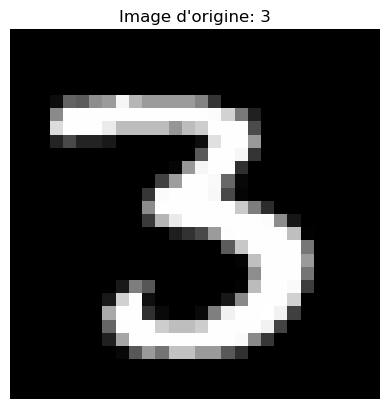
\includegraphics[width=1.0\linewidth]{Images/MNIST-3-7-origine}
				\label{fig:MNIST-3-7-origine}
			\end{figure}						
		\end{column}
		\begin{column}{0.25\textwidth}
			\begin{figure}
				\centering
				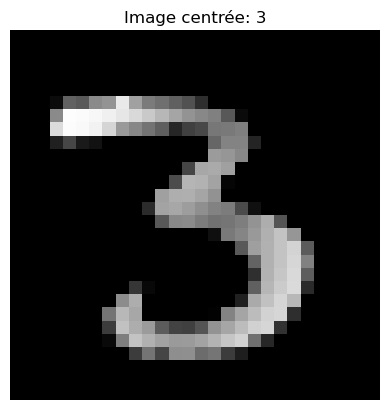
\includegraphics[width=1.0\linewidth]{Images/MNIST-3-7-centree}
				\label{fig:MNIST-3-7-centree}
			\end{figure}						
		\end{column}
		\begin{column}{0.25\textwidth}
			\begin{figure}
				\centering
				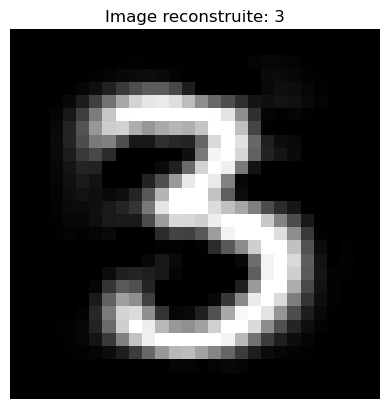
\includegraphics[width=1.0\linewidth]{Images/MNIST-3-7-reconstruite}
				\label{fig:MNIST-3-7-reconstruite}
			\end{figure}						
		\end{column}
		\begin{column}{0.25\textwidth}
			\begin{figure}
				\centering
				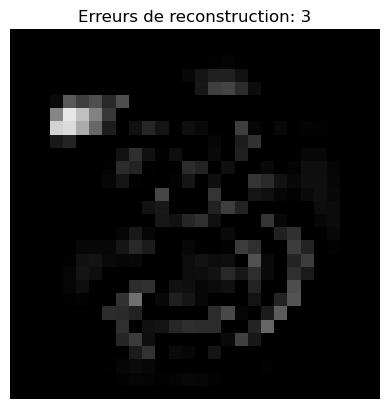
\includegraphics[width=1.0\linewidth]{Images/MNIST-3-7-erreur}
				\label{fig:MNIST-3-7-erreur}
			\end{figure}						
		\end{column}
	\end{columns}
\end{frame}

\begin{frame}{Retaining the Top 4 Components}
	In this extreme case, only 4 components are retained. We can now clearly see a sharp "3" silhouette in the error matrix. The reconstructed image no longer closely resembles a "3". Too much critical structural information has been lost by compressing the image so aggressively:
	\begin{columns}
		\begin{column}{0.25\textwidth}
			\begin{figure}
				\centering
				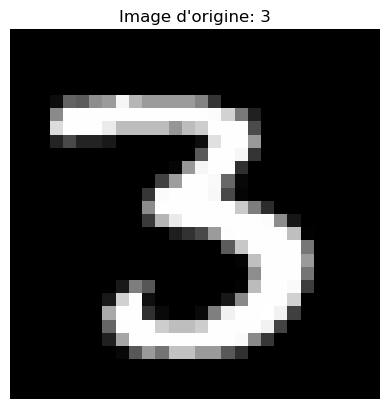
\includegraphics[width=1.0\linewidth]{Images/MNIST-3-2-origine}
				\label{fig:MNIST-3-2-origine}
			\end{figure}						
		\end{column}
		\begin{column}{0.25\textwidth}
			\begin{figure}
				\centering
				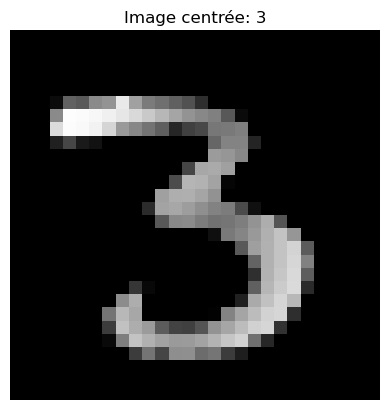
\includegraphics[width=1.0\linewidth]{Images/MNIST-3-2-centree}
				\label{fig:MNIST-3-2-centree}
			\end{figure}						
		\end{column}
		\begin{column}{0.25\textwidth}
			\begin{figure}
				\centering
				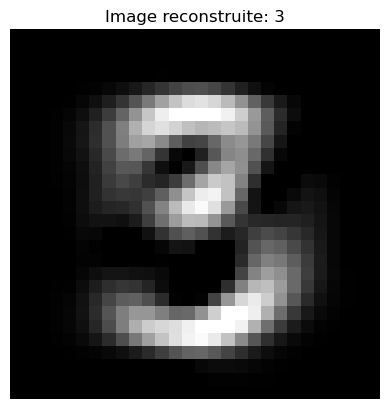
\includegraphics[width=1.0\linewidth]{Images/MNIST-3-2-reconstruite}
				\label{fig:MNIST-3-2-reconstruite}
			\end{figure}						
		\end{column}
		\begin{column}{0.25\textwidth}
			\begin{figure}
				\centering
				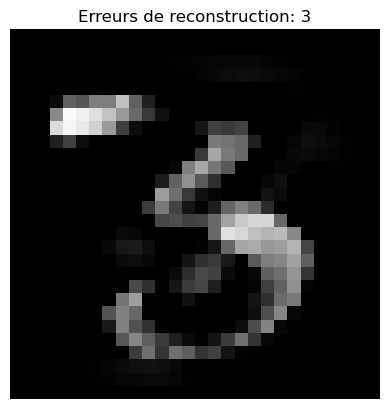
\includegraphics[width=1.0\linewidth]{Images/MNIST-3-2-erreur}
				\label{fig:MNIST-3-2-erreur}
			\end{figure}						
		\end{column}
	\end{columns}
\end{frame}